\chapter{Evaluation}\label{chap:evaluation}

To prove that our technique is beneficial, we conduct a standard empirical evaluation on PO domains and compare the runtime of a state-of-the-art planning system on the original problem vs. the transformed problem. All problems are taken from two benchmark sets prepared for 2020 IPC. The first set\footnote{\url{https://github.com/panda-planner-dev/ipc2020-domains/tree/master/partial-order}} was used in the partially ordered track in the 2020 IPC benchmark, while the second set\footnote{\url{https://github.com/panda-planner-dev/domains/tree/master/partial-order}} went un-used for various reasons. Each problem has the standard IPC time limit of 30 minutes. Where grounding and pre-processing is needed, the time to do this is included as part of the 'solving' time required. Since the pre-processing may \emph{potentially} remove all solutions, where the planning system can prove that the pre-processing renders a problem unsolvable, we use the remaining time to solve the original problem.

\section{Hardware and Planning Systems}
The empirical evaluation was conducted on a machine with 30GiB of memory and 4 vCPUs, each with 2 GiB RAM.  We use the $panda_{\pi}$ solver by \citep{useClassicalHuristicICAPS18,useClassicalHeuristicIJCAI19,progressionsearchJAIR20} on the configuration of Greedy best first search with visited lists. We try this search with 4 different RC-heuristics: FF \cite{FF}, Add \cite{Add}, Filter \cite{useClassicalHuristicICAPS18} and Landmark-cut \cite{LM-Cut}.

We compare the performance of these 4 planner settings on the original problem and the pre-processed problem.
We also try the Lilotane planner \cite{Lilotane}, which is specialised for TOHTN problems. For panda$_{pi}$, the same setting is used for re-runs. For Lilotane, re-runs use panda$_{pi}$ on the best setting (Add heuristic) to solve the original PO version of the problem.

%VCPUs  : 4 \newline
%Memory : 8GB, OR 8192(MB) \newline
%Disk   : 30GB \newline
%RAM per VCPU; 2GB \newline
%CPU Shares: 256 \newline

\section{Results}


\begin{table}[H]
	\setlength{\tabcolsep}{2.5pt} 
	\caption{IPC score, with and without pre-processing, for all planners. If any problems in that domain were proven unsolvable by TO, a number in brackets beside domain name shows how many.} \label{tabIPC} 
	\scalebox{0.8}{ 
		\begin{tabular}{lccccccccccccccccccl} 
\toprule 
  && \multicolumn{2}{c}{rc2(Add)} & \multicolumn{2}{c}{rc2(Filter)} & \multicolumn{2}{c}{rc2(FF)} & \multicolumn{2}{c}{rc2(LMC)} & \multicolumn{2}{c}{Lilotane} \\ 
\cmidrule(lr){3-4} \cmidrule(lr){5-6} \cmidrule(lr){7-8} \cmidrule(lr){9-10} \cmidrule(lr){11-12}  
 & max &PO & TO & PO & TO & PO & TO & PO &\multicolumn{2}{c}{ TO  } \\ 
\midrule 
Barman-BDI & 1 & 0.08 & \textbf{0.4} & 0.07 & \textbf{0.34} & 0.07 & \textbf{0.36} & 0.05 & \textbf{0.22} &\multicolumn{2}{c}{ \textbf{0.72}  } \\ 
Monroe Fully Observ.$^{2}$ & 1 & \textbf{0.56} & 0.45 & \textbf{0.31} & 0.3 & \textbf{0.46} & 0.41 & \textbf{0.22} & 0.18 &\multicolumn{2}{c}{ 0.54  } \\ 
Monroe Part. Observ.$^{2}$ & 1 & \textbf{0.31} & 0.25 & \textbf{0.13} & 0.11 & \textbf{0.31} & 0.26 & \textbf{0.17} & 0.14 &\multicolumn{2}{c}{ \textbf{0.63}  } \\ 
PCP$^{17}$ & 1 & \textbf{0.82} & \textbf{0.82} & \textbf{0.82} & \textbf{0.82} & \textbf{0.82} & \textbf{0.82} & \textbf{0.82} & \textbf{0.82} &\multicolumn{2}{c}{ 0.0  } \\ 
Rover & 1 & 0.29 & \textbf{0.95} & 0.14 & \textbf{0.52} & 0.2 & \textbf{0.78} & 0.16 & \textbf{0.48} &\multicolumn{2}{c}{ \textbf{0.97}  } \\ 
Satellite & 1 & 0.91 & \textbf{1.0} & 0.76 & \textbf{1.0} & 0.99 & \textbf{1.0} & 0.89 & \textbf{0.99} &\multicolumn{2}{c}{ \textbf{1.0}  } \\ 
SmartPhone$^{1}$ & 1 & \textbf{0.71} & \textbf{0.71} & 0.69 & \textbf{0.71} & \textbf{0.71} & \textbf{0.71} & \textbf{0.71} & \textbf{0.71} &\multicolumn{2}{c}{ 0.14  } \\ 
Transport & 1 & 0.24 & \textbf{0.61} & 0.04 & \textbf{0.05} & 0.27 & \textbf{0.32} & 0.12 & \textbf{0.2} &\multicolumn{2}{c}{ \textbf{0.78}  } \\ 
UM-Translog$^{1}$ & 1 & \textbf{1.0} & \textbf{1.0} & \textbf{1.0} & \textbf{1.0} & \textbf{1.0} & \textbf{1.0} & \textbf{1.0} & \textbf{1.0} &\multicolumn{2}{c}{ 0.92  } \\ 
Woodworking$^{2}$ & 1 & 0.38 & \textbf{0.58} & 0.2 & \textbf{0.41} & 0.36 & \textbf{0.57} & 0.27 & \textbf{0.39} &\multicolumn{2}{c}{ 0.2  } \\ 
\midrule 
Monroe & 1 & \textbf{0.77} & 0.69 & \textbf{0.5} & 0.47 & \textbf{0.75} & 0.71 & \textbf{0.53} & \textbf{0.53} &\multicolumn{2}{c}{ \textbf{0.96}  } \\ 
SmartPhone$^{1}$ & 1 & \textbf{0.71} & \textbf{0.71} & 0.69 & \textbf{0.71} & \textbf{0.71} & \textbf{0.71} & \textbf{0.71} & \textbf{0.71} &\multicolumn{2}{c}{ 0.14  } \\ 
Zenotravel & 1 & \textbf{1.0} & \textbf{1.0} & 0.63 & \textbf{1.0} & \textbf{1.0} & \textbf{1.0} & 0.83 & \textbf{1.0} &\multicolumn{2}{c}{ \textbf{1.0}  } \\ 
\midrule 
IPC score & 13 & 7.8 & \textbf{9.2} & 6.0 & \textbf{7.5} & 7.7 & \textbf{8.7} & 6.5 & \textbf{7.4} &\multicolumn{2}{c}{ 8.0  } \\ 
\bottomrule 
 \end{tabular} 

	}
\end{table}



\begin{table}[H]
	\setlength{\tabcolsep}{2.5pt} 
	\caption{Coverage, with and without pre-processing, for all planners. If any problems in that domain were proven unsolvable by TO, a number in brackets beside domain name shows how many.}\label{tabcoverage} 
	\scalebox{0.8}{ 
		\begin{tabular}{lccccccccccccccccccl} 
\toprule 
  && \multicolumn{2}{c}{rc2(Add)} & \multicolumn{2}{c}{rc2(Filter)} & \multicolumn{2}{c}{rc2(FF)} & \multicolumn{2}{c}{rc2(LMC)} & \multicolumn{2}{c}{Lilotane} \\ 
\cmidrule(lr){3-4} \cmidrule(lr){5-6} \cmidrule(lr){7-8} \cmidrule(lr){9-10} \cmidrule(lr){11-12}  
 & max &PO & TO & PO & TO & PO & TO & PO &\multicolumn{2}{c}{ TO  } \\ 
\midrule 
Barman-BDI & 20 & 3.0 & \textbf{10.0} & 3.0 & \textbf{10.0} & 3.0 & \textbf{10.0} & 2.0 & \textbf{9.0} &\multicolumn{2}{c}{ \textbf{17.0}  } \\ 
 Monroe Fully Observ.$^{2}$ & 25 & \textbf{25.0} & \textbf{25.0} & 18.0 & \textbf{25.0} & 22.0 & \textbf{25.0} & 15.0 & \textbf{16.0} &\multicolumn{2}{c}{ 18.0  } \\ 
 Monroe Part. Observ.$^{2}$ & 24 & \textbf{14.0} & \textbf{14.0} & \textbf{7.0} & \textbf{7.0} & 14.0 & \textbf{15.0} & \textbf{10.0} & \textbf{10.0} &\multicolumn{2}{c}{ \textbf{20.0}  } \\ 
PCP$^{17}$ & 17 & \textbf{14.0} & \textbf{14.0} & \textbf{14.0} & \textbf{14.0} & \textbf{14.0} & \textbf{14.0} & \textbf{14.0} & \textbf{14.0} &\multicolumn{2}{c}{ 0.0  } \\ 
Rover & 20 & 6.0 & \textbf{20.0} & 4.0 & \textbf{14.0} & 4.0 & \textbf{19.0} & 4.0 & \textbf{14.0} &\multicolumn{2}{c}{ \textbf{20.0}  } \\ 
Satellite & 25 & 24.0 & \textbf{25.0} & 22.0 & \textbf{25.0} & \textbf{25.0} & \textbf{25.0} & 24.0 & \textbf{25.0} &\multicolumn{2}{c}{ \textbf{25.0}  } \\ 
SmartPhone$^{1}$ & 7 & \textbf{5.0} & \textbf{5.0} & \textbf{5.0} & \textbf{5.0} & \textbf{5.0} & \textbf{5.0} & \textbf{5.0} & \textbf{5.0} &\multicolumn{2}{c}{ 1.0  } \\ 
Transport & 40 & 12.0 & \textbf{28.0} & \textbf{2.0} & \textbf{2.0} & 13.0 & \textbf{14.0} & 7.0 & \textbf{12.0} &\multicolumn{2}{c}{ \textbf{35.0}  } \\ 
UM-Translog$^{1}$ & 22 & \textbf{22.0} & \textbf{22.0} & \textbf{22.0} & \textbf{22.0} & \textbf{22.0} & \textbf{22.0} & \textbf{22.0} & \textbf{22.0} &\multicolumn{2}{c}{ 21.0  } \\ 
Woodworking$^{2}$ & 30 & 13.0 & \textbf{19.0} & 7.0 & \textbf{15.0} & 12.0 & \textbf{20.0} & 9.0 & \textbf{15.0} &\multicolumn{2}{c}{ 6.0  } \\ 
\midrule 
 Monroe & 100 & 96.0 & \textbf{100.0} & 79.0 & \textbf{88.0} & 92.0 & \textbf{100.0} & 81.0 & \textbf{90.0} &\multicolumn{2}{c}{ \textbf{100.0}  } \\ 
SmartPhone$^{1}$ & 7 & \textbf{5.0} & \textbf{5.0} & \textbf{5.0} & \textbf{5.0} & \textbf{5.0} & \textbf{5.0} & \textbf{5.0} & \textbf{5.0} &\multicolumn{2}{c}{ 1.0  } \\ 
Zenotravel & 5 & \textbf{5.0} & \textbf{5.0} & \textbf{5.0} & \textbf{5.0} & \textbf{5.0} & \textbf{5.0} & \textbf{5.0} & \textbf{5.0} &\multicolumn{2}{c}{ \textbf{5.0}  } \\ 
\midrule 
 Coverage & 342 & 244.0 & \textbf{292.0} & 193.0 & \textbf{237.0} & 236.0 & \textbf{279.0} & 203.0 & \textbf{242.0} &\multicolumn{2}{c}{ 269.0  } \\ 
Norm. coverage & 13 & 8.94 & \textbf{10.67} & 7.57 & \textbf{9.17} & 8.71 & \textbf{10.34} & 7.81 & \textbf{9.16} &\multicolumn{2}{c}{ 8.72  } \\ 
IPC score & 13 & 7.8 & \textbf{9.2} & 6.0 & \textbf{7.5} & 7.7 & \textbf{8.7} & 6.5 & \textbf{7.4} &\multicolumn{2}{c}{ 8.0  } \\ 
\bottomrule 
 \end{tabular} 

	}
\end{table}

\begin{figure}
	\floatbox[{\capbeside\thisfloatsetup{capbesideposition={left,center},capbesidewidth=6cm}}]{figure}[\FBwidth]
	{\caption{Percentage of problems for which linearized problems is faster to solve, for problems that took at least $\mathit{x}$ seconds to solve, with $\mathit{x}$  being the value on the x-axis. \\ \label{faster}}}
	{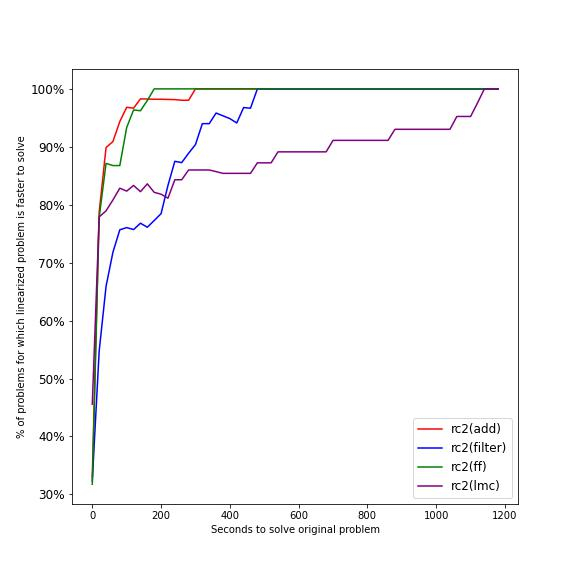
\includegraphics[width=5cm]{figures/faster_to_solve_m.jpg}}
\end{figure}

% 'UM-Translog': 1, 'Monroe-Fully-Observable': 2, 'Woodworking': 2, 'Monroe-Partially-Observable': 2, 'PCP': 17, 'SmartPhone': 1}

\begin{figure}[H]
	\caption{Comparison of time to solve PO and TO problems, for each $panda_{\pi}$ setting} \label{RuntimevsSolved}
	\begin{subfigure}{6cm}
		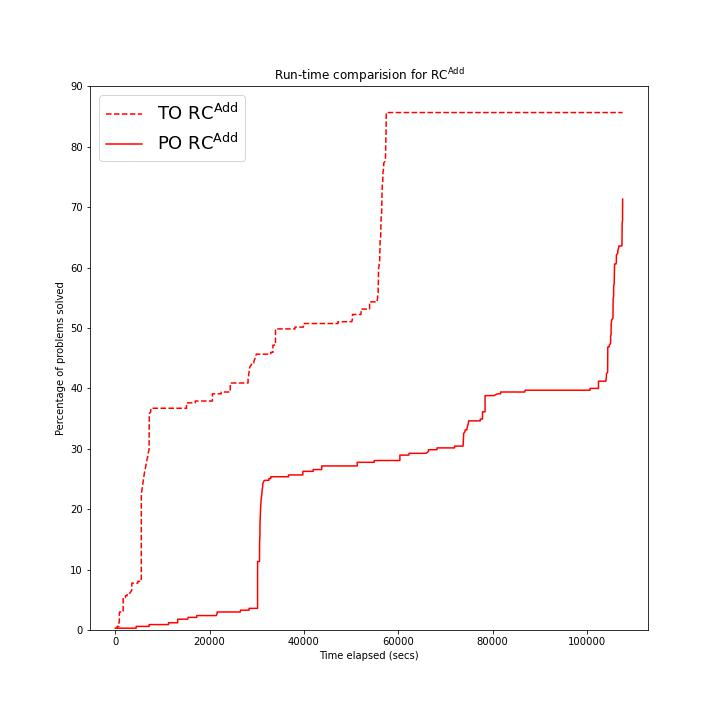
\includegraphics[width=5cm]{figures/Runtime comparisionRC(Add).jpg}	
		\caption{Using heuristic RC\textsuperscript{add}}	
	\end{subfigure}
	\begin{subfigure}{6cm}
		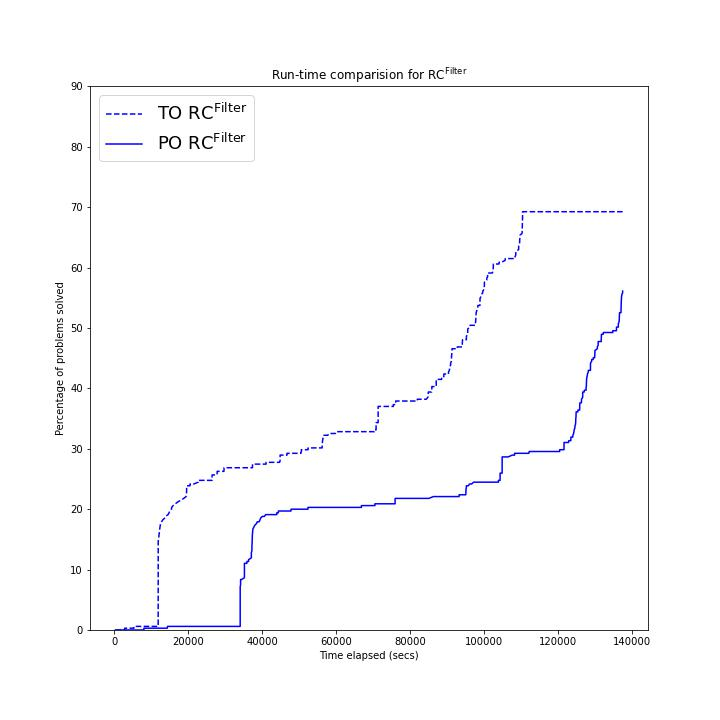
\includegraphics[width=5cm]{figures/Runtime comparisionRC(Filter).jpg}	
		\caption{Using heuristic RC\textsuperscript{Filter}}
	\end{subfigure}
	
	\begin{subfigure}{6cm}
		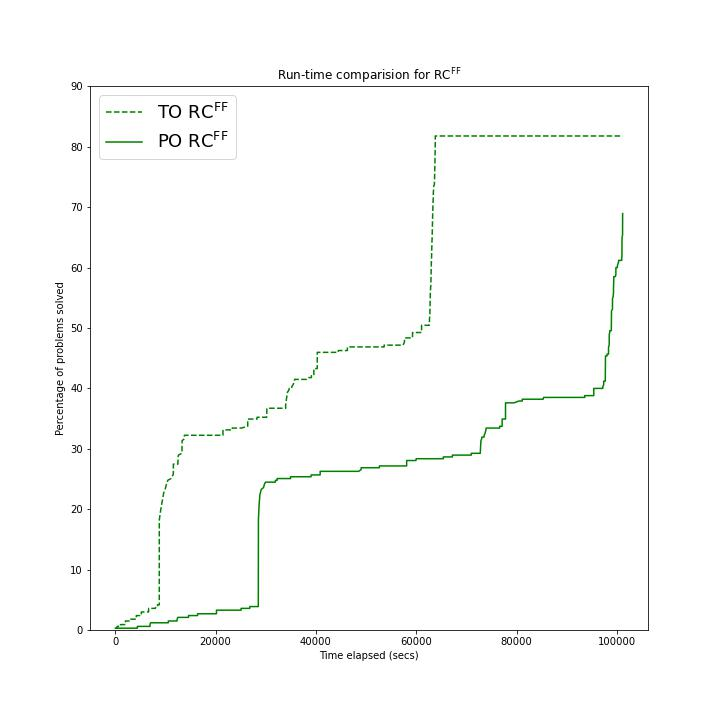
\includegraphics[width=5cm]{figures/Runtime comparisionRC(FF).jpg}	
		\caption{Using heuristic RC\textsuperscript{FF}}	
	\end{subfigure}
	\begin{subfigure}{6cm}
		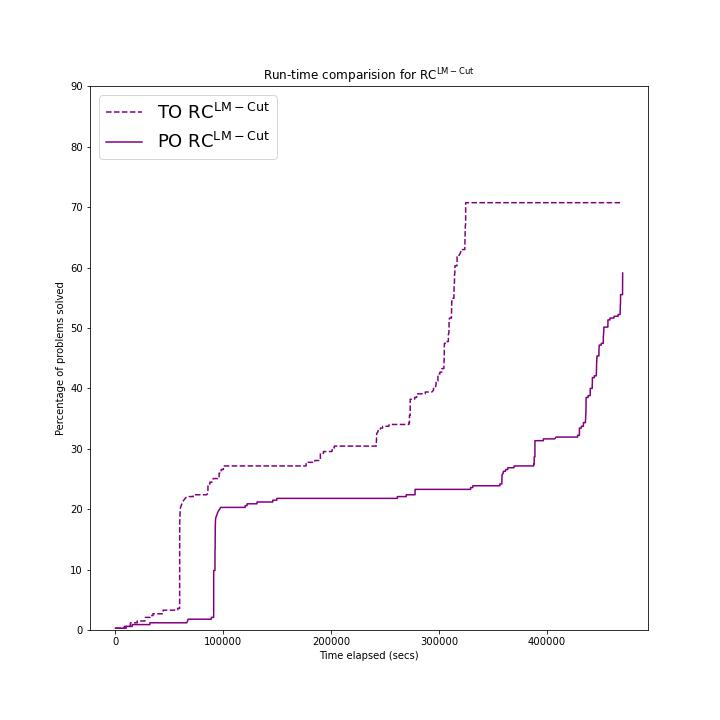
\includegraphics[width=5cm]{figures/Runtime comparisionRC(LM-Cut).jpg}
		\caption{Using heuristic RC\textsuperscript{LM-Cut}}		
	\end{subfigure}
\end{figure}



\newpage

\section{Analysis}

Table~\ref{tabIPC} and \ref{tabcoverage} shows that the IPC score and coverage when pre-processing is overall significantly better than when not using pre-processing. 

However in some domains there is minimal gain, if any at all. This seems to be because some domains are dominated by small problems. E.g.\ 14 of the 17 PCP problems take less than 0.5 seconds to solve. For very small problems, the pre-processing still takes time, but very little improvement can be gained in the actual solving time. In fact, a second of pre-processing time for a problem that only takes a few seconds to solve will worsen IPC score. 

On the other hand, big problems experience significant improvement, enough to make problems solvable within the time limit where they were previously too memory or time intensive. We can see that difference in domains like Rover and Barman-BDI, where there is significant space to improve on coverage/speed.

\begin{table}[t] 
	\setlength{\tabcolsep}{2.5pt} 
\caption{With re-run policy}\label{tabsummary2} 
\scalebox{0.85}{
 \begin{tabular}{lccccccl} 
\toprule 
&   & Solved & Out of Memory & Timeout & Unsolvable &  \\ 
\midrule
  \multirow{3}*{RC\textsuperscript{add}}& TO & 287 & 27 & 21 & 0  \\ 
& PO & 239 & 65 & 31 & 0  \\ 
& Either & 287 & 72 & 40 & 0  \\ 
\midrule 
 \multirow{3}*{RC\textsuperscript{Filter}}& TO & 232 & 85 & 18 & 0  \\ 
& PO & 188 & 115 & 32 & 0  \\ 
& Either & 232 & 125 & 35 & 0  \\ 
\midrule 
 \multirow{3}*{RC\textsuperscript{FF}}& TO & 274 & 41 & 20 & 0  \\ 
& PO & 231 & 76 & 28 & 0  \\ 
& Either & 274 & 85 & 37 & 0  \\ 
\midrule 
 \multirow{3}*{RC\textsuperscript{LM-Cut}}& TO & 237 & 6 & 92 & 0  \\ 
& PO & 198 & 11 & 126 & 0  \\ 
& Either & 237 & 12 & 126 & 0  \\ 
\midrule 
Lilotane & TO & 268 & 67 & 0 & 0  \\
\bottomrule 
 \end{tabular} 
}
\end{table} 

\begin{table}[t]
	\setlength{\tabcolsep}{2.5pt} 
\caption{Without re-run policy}\label{tabsummary1} 
\scalebox{0.85}{
 \begin{tabular}{lccccccl} 
\toprule 
&   & Solved & Out of Memory & Timeout & Unsolvable &  \\ 
\midrule
\multirow{3}*{RC\textsuperscript{add}}& TO & 266 & 24 & 20 & 25  \\ 
& PO & 239 & 65 & 31 & 0  \\ 
& Either & 287 & 72 & 40 & 25  \\ 
\midrule 
 \multirow{3}*{RC\textsuperscript{Filter}}& TO & 212 & 80 & 18 & 25  \\ 
& PO & 188 & 115 & 32 & 0  \\ 
& Either & 232 & 125 & 35 & 25  \\ 
\midrule 
 \multirow{3}*{RC\textsuperscript{FF}}& TO & 253 & 38 & 19 & 25  \\ 
& PO & 231 & 76 & 28 & 0  \\ 
& Either & 274 & 85 & 37 & 25  \\ 
\midrule 
 \multirow{3}*{RC\textsuperscript{LM-Cut}}& TO & 217 & 2 & 91 & 25  \\ 
& PO & 198 & 11 & 126 & 0  \\ 
& Either & 237 & 12 & 126 & 25  \\ 
\midrule 
Lilotane & TO & 268 & 67 & 0 & 0  \\
\bottomrule 
 \end{tabular}
} 
\end{table} 


Table~\ref{tabsummary1} and Table~\ref{tabsummary2} summarises the results of our empirical evaluation on the IPC 2020 benchmarks. The \enquote{unsolvable} columns refer to problems that the solver determined to have no solutions. 
Note that panda$_\pi$ planning system wants a grounded representation, while Lilotane wants a lifted representation. Therefore, while a linearized, lifted problem is fed to both, panda$_\pi$ works grounds the problem before solving.
%\todo{Talk about difference between linearize $\to$ ground, and ground $\to$ linearize?}
%\todo{Lilotane CAN prove unsolvable problems - update tables \ref{tabsummary1} and \ref{tabsummary2}  }
%\todo{run HyperTensioN on lifted problems?}

The PCP domain in particular was rendered unsolvable for all instances.  In Table~\ref{tabIPC} and Table~\ref{tabcoverage}, $\text{PCP}^{17}$ indicates that 17 PCP problems were unsolvable. So all 14 problems \enquote{solved} in the TO context was from re-running the planner on the original problem using the remaining time. Incidentally, the exact same problems were proven unsolvable for all planners.

The PCP domain defines the post-correspondence problem, which is known to be undecidable. Totally ordered HTN planning problems are always decidable \cite{ErolHTNExpressivity}, meaning it's a direct consequence that these problem instances are unsolvable without task interleaving. In this specific case, the PCP problems designed for the IPC benchmark are known to be unsolvable without interleaving \cite{PCPDomain}. Table~\ref{tabsummary2} shows the results on the default setting, when allowing the planner to try solving the original problem as a back-up plan when the linearized problem fails. 

%Lilotane \cite{Lilotane}, the runner-up for the totally ordered track in the 2020 IPC competition, can prove that a problem is unsolvable, \todo{though it is notably less successful at doing so
%	than $panda_{pi}$ planner}

%Lilotane is excluded from Table~\ref{tabsummary2} as it cannot prove a problem is unsolvable, and so cannot use the re-run policy. instead. Table~\ref{tabsummary1} shows results without the default back-up strategy.  % the planner moves on to the next problem immediately after the linearized approach for a problem fails.
%  This means that if we could convert such that it retained a solution, we would be turning an undecidable problem into a decidable one -- in other words impossible. A totally ordered problem just does not have the expressive power.


From Table ~\ref{tabsummary2} and \ref{tabsummary1} we can see that this processing means that many more problems can be solved in the time limit, where previously they were too computation-intensive, and very few problems (primarily problems for which interleaving is required for all solutions) become unsolvable due to the transformation. Despite the fact that none of the instances can be linearized without cycle-breaking, only 25/274 of linearized problems are unsolvable, 17 of which are from the PCP domain, where a solvable linearization does not exist.
